\documentclass{article}


\usepackage{amsthm,amsmath}
\usepackage{amssymb}
\usepackage{dsfont}
\usepackage[utf8]{inputenc}
\usepackage{url}
\usepackage{color}
\usepackage{xspace}
\usepackage{graphicx}
\usepackage{hyperref}
\usepackage{pdfpages}
\usepackage{relsize}
\usepackage{siunitx}
% \def\includegraphic[#1]{}
% \def\includegraphics[#1]{}

\graphicspath{{figures/}{./}}

\DeclareMathOperator*{\median}{median}
\DeclareMathOperator*{\card}{card}

\newcommand*{\eg}{e.g.,\@\xspace}
\newcommand*{\ie}{i.e.,\@\xspace}
\newcommand*{\vs}{vs.\@\xspace}


\newcommand{\Card}{\mathrm{card}}

\newcommand{\ml}[1]{\textcolor{blue}{ML: #1}\xspace}
\newcommand{\vl}[1]{\textcolor{red}{VL: #1}\xspace}
\newcommand{\ja}[1]{\textcolor{purple}{JA: #1}\xspace}



\title{Judgments of timbre similarity \\ across instruments and playing techniques}
\author{Mathieu Lagrange, Vincent Lostanlen, Joakim And\'{e}n}
\date{\today}

\begin{document}

\maketitle


\begin{figure}
\center
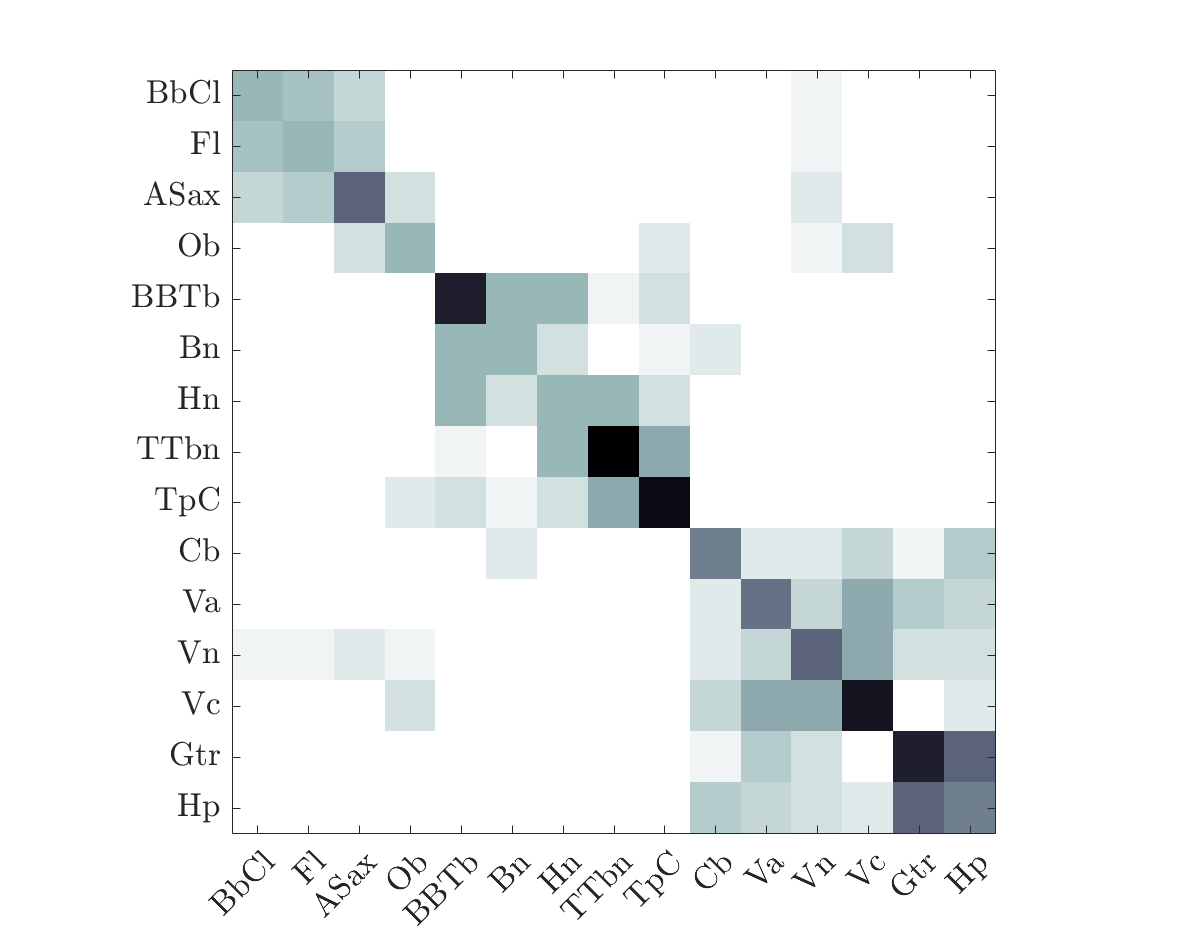
\includegraphics[width = 0.85\textwidth]{consensusVsI.png}
\caption{
Matrix $\mathbf{\widetilde{A}}_{\mathcal{I}}$ of perceived timbre similarities between instruments from our dataset of $N=78$. samples.
Darker shades indicate higher frequencies of co-occurrence in the cluster graph $\mathcal{G}_0$ (see Equation \ref{eq:instrument-similarity}), obtained from a consensus of $K=31$ subjects.
The rows and columns in $\mathbf{\widetilde{A}}_{\mathcal{I}}$ were re-arranged according to Ward's minimum variance method.
Observe that the block diagonal structure in $\mathbf{\widetilde{A}}_{\mathcal{I}}$ reflects an organological taxonomy of musical instruments: woodwinds, brass, and strings.
}
\label{fig:consensusVsI}
\end{figure}

\begin{figure}
\center
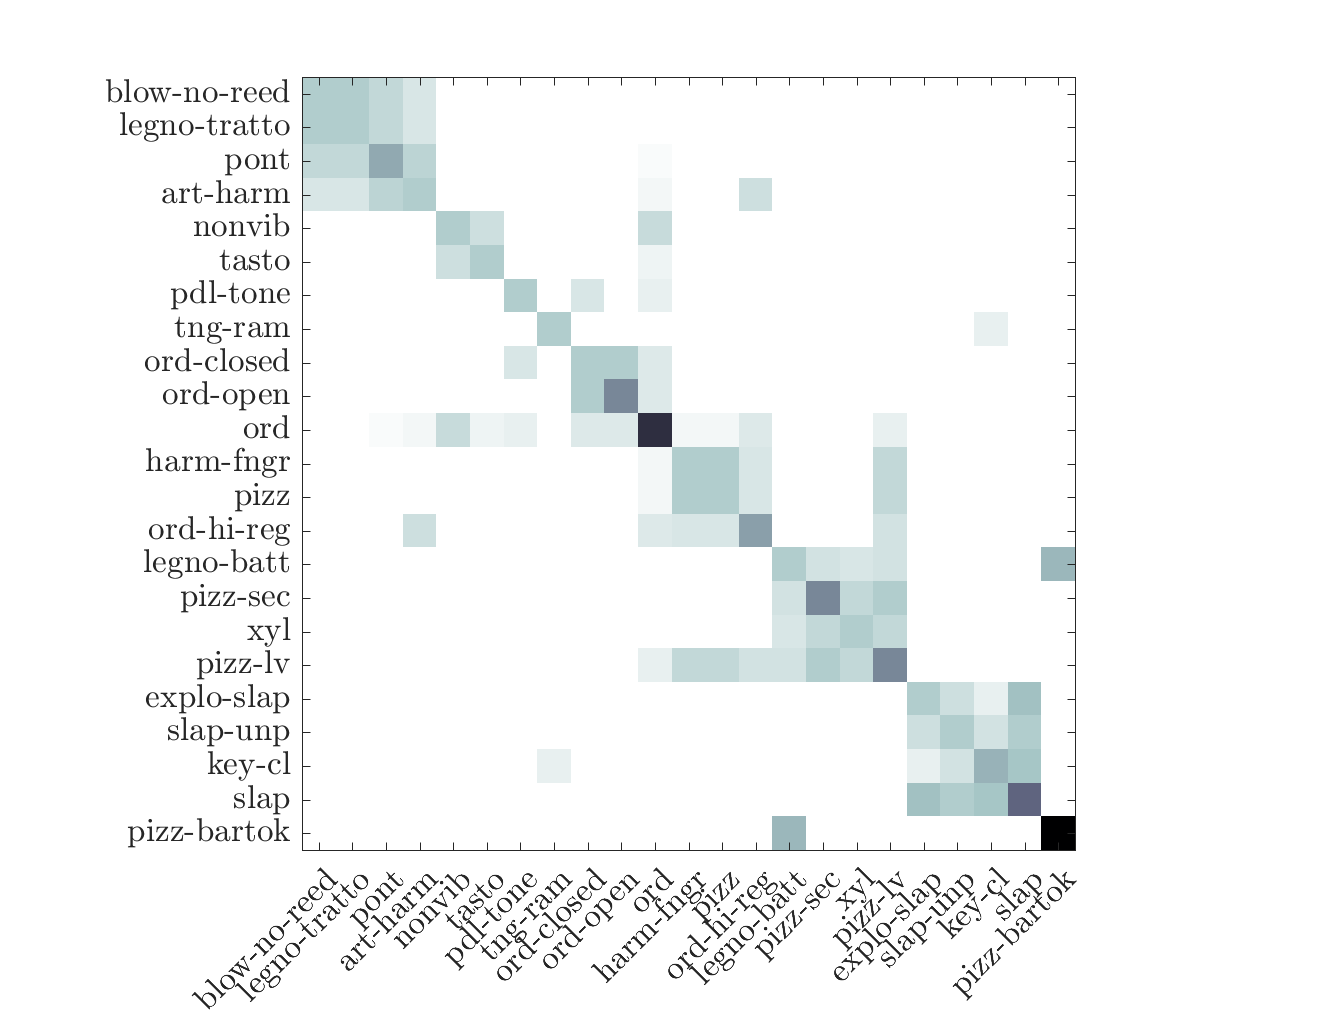
\includegraphics[width = 0.85\textwidth]{consensusVsPt.png}
\caption{
Matrix $\mathbf{\widetilde{A}}_{\mathcal{T}}$ of perceived timbre similarities between playing techniques from our dataset of $N=78$ samples.
Darker shades indicate higher frequencies of co-occurrence in the cluster graph $\mathcal{G}_0$ (see Equation \ref{eq:technique-similarity}), obtained from a consensus of $K=31$ subjects.
The rows and columns in $\mathbf{\widetilde{A}}_{\mathcal{T}}$ were re-arranged according to Ward's minimum variance method.
%TODO add a double arrow?
% rough <-- soft --> rough
% sustained <-- "ordinary" --> percussive
}
\label{fig:consensusVsPt}
\end{figure}

\subsection*{Inter-instrument similarity}

We ask whether human listeners tend to cluster audio samples by instrument.
To answer this question, we derive from the consensus clustering graph $\mathcal{G}_0$ an instrument-wise similarity matrix $\mathbf{A}_{\mathcal{I}}$ whose rows and columns are defined on the finite set $\mathcal{I}$ of instruments.
For every instrument--instrument pair $(i,j)$, we set the value of $\mathbf{A}_{\mathcal{I}}$ at row $i$ and column $j$ equal to the number of edges in $\mathcal{G}_0$ connecting IMTs from instruments $i$ and $j$, renormalized by the number of IMT samples from either instrument $i$ or instrument $j$.

Let us denote the existence of an edge in $\mathcal{G}_0$ connecting two IMT samples $m$ and $n$ by the binary relation $m \overset{\mathcal{G}_0}{\sim} n$.
The mathematical definition of the matrix $\mathbf{A}_{\mathcal{I}}$ is:
\begin{equation}
\mathbf{A}_{\mathcal{I}}(i,j) = \dfrac{
\,\Card \big\{ (m, n) \,\vert\, \mathrm{Instrument}(m)=i ; \mathrm{Instrument}(n)=j ; m \overset{\mathcal{G}_0}{\sim} n \big\}
}{
\Card \big\{n \,\vert\, \mathrm{Instrument}(n) \in \{ i, j \} \big\}
}.
\label{eq:instrument-similarity}
\end{equation}

Then, we run Ward's method \cite{ward1963jasa} to cluster instruments in $\mathcal{I}$ according to the similarity matrix $\mathbf{A}_{\mathcal{I}}$.
This method yields a permutation $\sigma_{\mathcal{I}}: \mathcal{I} \rightarrow \mathcal{I}$ of the rows and columns in $\mathbf{A}_{\mathcal{I}}$ such that the distance $\vert \sigma_{\mathcal{I}}(i) - \sigma_{\mathcal{I}}(j) \vert$ after permutation is small if and only if the similarity $\mathbf{A}_{\mathcal{I}}(i, j)$ is large.
Figure \ref{fig:consensusVsI} displays the rearranged similarity matrix $\widetilde{\mathbf{A}}_{\mathcal{I}} : (i,j)\in \mathcal{I}^2 \mapsto \mathbf{A}_{\mathcal{I}}(\sigma_{\mathcal{I}}^{-1}(i), \sigma_{\mathcal{I}}^{-1}(j))$ as a result of such agglomerative hierarchical clustering procedure. % \ja wants to remove this equation

Interestingly, the matrix $\widetilde{\mathbf{A}}_{\mathcal{I}}$ exhibits a block diagonal structure, which roughly reflects the classical taxonomy of musical instruments: four woodwinds (BbCl, Fl, ASax, Ob) are clustered together, followed by a cluster containing one woodwind (Bn) and four brass (BBTb, Hn, TTbn, and TpC), followed by a cluster of all strings (Cb, Va, Vn, Vc, Gtr, Hp).
Furthermore, the largest cross-instrument similarity arises for the only pair of purely plucked instruments, namely, harp and guitar.


\subsection*{Inter-technique similarity}
From the consensus clustering graph $\mathcal{G}_0$, we also derive a technique-wise similarity matrix $\mathbf{A}_{\mathcal{T}}$ whose rows and columns are defined on the finite set $\mathcal{T}$ of playing techniques.
As for $\mathbf{A}_{\mathcal{I}}$, we define the similarity between any two playing techniques $u$ and $v$ in $\mathcal{T}$ as the following ratio of set cardinalities:
\begin{equation}
\mathbf{A}_{\mathcal{T}}(u,v) = \dfrac{
\,\Card \big\{ (m, n) \,\vert\, \mathrm{Technique}(m)=u ; \mathrm{Technique}(n)=v ; m \overset{\mathcal{G}_0}{\sim} n \big\}
}{
\Card \big\{n \,\vert\, \mathrm{Technique}(n) \in \{ u, v \} \big\}
}.
\label{eq:technique-similarity}
\end{equation}
Again, we run Ward's method to cluster playing techniques in $\mathcal{T}$ according to their similarity $\mathbf{A}_{\mathcal{T}}$.
Figure \ref{fig:consensusVsPt} displays the rearranged similarity matrix $\widetilde{\mathbf{A}}_{\mathcal{T}} : (u,v)\in \mathcal{T}^2 \mapsto \mathbf{A}_{\mathcal{T}}(\sigma_{\mathcal{T}}^{-1}(u), \sigma_{\mathcal{T}}^{-1}(v))$.

The block diagonal structure of the matrix $\widetilde{\mathbf{A}}_{\mathcal{T}}$ is less salient than in $\widetilde{\mathbf{A}}_{\mathcal{I}}$.
Nevertheless, these clusters correspond to some basic attributes of qualitative timbre: by and large, the top-left region of the matrix contains sustained sounds whereas the bottom-right region contains percussive sounds.
Interestingly, the ordinary technique (\texttt{ord}) appears at the center of the matrix, \ie{} at the intersection between sustained sounds and percussive sounds.
This is because the notion of ``ordinariness'' does not prescribe the same gesture for all instruments: \eg{} an ordinary guitar sound is expected to be percussive whereas an ordinary flute sound is expected to be sustained.


\end{document}
